\title{Fuzz Testing with Inferred Attribute Grammars}
\author{
        Tim Henderson\\
        Case Western Reserve University\\
}
\date{\today}

\maketitle

\begin{abstract}
Blackbox Fuzzing, a type automated dynamic test generation, has been heavily
used to find security vulnerabilities and faults in software. We propose a new
form of Blackbox Fuzzing: Inferred Attribute Grammar Fuzzing. Attribute grammars
have a long distinguished history in specifying context sensitive restrictions to
context free languages. We use them here to assist with generating correct
randomized inputs for programs with structured input languages.  Attribute
Grammars are time consuming to write by hand, and a grammar for the input
language of the program under test may not be available. Therefore, we
present a multi-step approach to constructing inferred Attribute Grammars useful
for Fuzz Testing. Our approach assumes the existence of a large set of
operational inputs.
\end{abstract}
\vspace{.5in}


\section{Introduction}

Attribute Grammars were invented in the heady days of the late 1960's by Dr.
Knuth.\cite{Knuth1990} At the time the question on how to formally define the
semantics of a programming language had become a fashionable research topic.
Attribute grammars emerged as a popular way and remain important for such
purposes today. The key to their success is the ability to define context
sensitive semantics in languages. A common example, variable names must be
declared before use.

Input Languages to programs are often context sensitive. The obvious and natural
example is computer programming languages which encompass a wide variety of
useful programs. Web browsers, text editors, integrated development environments,
web servers, and game engines all make use of programming languages. Sometimes
exposing the languages to the end user for extensibility purposes. Other program
types have similarly complex input schemes often arising from natural world,
for example organic chemical structures.

Fuzzing, in particular ``Blackbox Fuzzing'' automatically generates test cases
for software. In the simplest formulation the test cases are little more than
random data. These types of tests produce poor coverage of the target program.
Context free grammar based fuzzing produces better results. However, context
free grammars are still unable to achieve good coverage of the entire target
program. 

Why do context free grammars fail when used to generate test cases for software
even when the grammar is known (and not inferred)? Context free grammars only
capture the syntax of the language and not the semantics. This means, the
language the program accepts as input is strictly a subset of the language the
CFG generates. Depending on the size of the gap between the CFG and the actual
language a random string generated from the CFG may only have a very small
chance of being in the language.


\section{Context Free Grammar Stats}
\label{cfgstats}
\subsection{Introduction}
Fuzzing with context free grammars is done by making choices. Specifically, a
rule needs to be chosen at each non-terminal, each of which includes additional
terminal and/or non-terminal symbols. Eventually, after making many choices, a
point is reached in where there is no other non-terminal left to choose rules
from and one is left with a string of terminal symbols.

The ``quality'' of the generated output depends upon the choices
which are made. Therefore, it is critical to have some sort of way of making
``good'' choices: some way other than simply choosing a random rule from a
non-terminal. This is where statistics come in.

If Fuzzbuzz is able to take in various tables of statistics then it will
inherently be able to make informed choices. For example, a basic statistics
table might include production probabilities. That is to say, given some
non-terminal and its set of rules, what are the probabilities for each rule?
Given the following simple grammar, the table would provide $\mathbb{P}[B]$,
$\mathbb{P}[C]$, and $\mathbb{P}[D]$ where $\mathbb{P}[B] + \mathbb{P}[C] +
\mathbb{P}[D] = 1$.

\begin{align*}
A &\rightarrow B \\
&\rightarrow C \\
&\rightarrow D \\
\end{align*}

\noindent
This is certainly much better than making random choices, but it is still
rather basic. We now present a literature review of picking rules given a CFG.

\subsection{Literature Review}

Maurer\cite{Maurer1990} gives a wide range of ideas for choosing rules. In his
paper, he describes a simple calculator grammar and then focuses on various
ways he could use the grammar to test his calculator program. He gives various
ideas for picking rules, though he does not go in depth as to whether following
them produces better results. He mentions how one possibility is to avoid
choosing the same rule twice, or how perhaps rules should be chosen in a
particular order. Maurer, however, focuses a lot on user customization,
something which we do not. For example, Maurer suggests altering the
probabilities manually (which he refers to as weights). He reasons that by
doing so, one can generate tests which focus more in a particular area that is
believed to have bugs.

Maurer also suggests keeping track of the number of bugs encountered when a
particular rule is chosen, and then auto adjusting the probabilities to favor
those rules which detect the most bugs. We found this to be an interesting
approach.

Sirer and Bershad\cite{Bershad1999} describe their experience with using
production grammars in order to test software. Their paper does not exactly
propose ways of using statistics to pick rules, though it does suggest other
criteria you can use in order to come to a decision. The authors were working
primarily with the Java programing language, and as such some of their ideas
cater to Java specifics, though are nevertheless interesting enough to be
mentioned in this paper.

One approach which Sirer and Bershad discussed was imposing a limit on how many
times specific grammar rules can be exercised. This is especially useful in
languages like Java that have structural limits such as code length per
method. The authors describe another way in which this can turn out to be
useful: if one wants to ensure that the program doesn't ``terminate early''
(i.e. that it is of a minimum length) is to, for example, set a limit on your
start symbol to 5000 and then a probability of zero on the production $S
\rightarrow \lambda$. This will ``force'' a stop rather than ``naturally''
stopping.

In addition to using production limits, Sirer and Bershad also mention how
probabilities are of good use and emphasize the usefulness of separating
probabilities from the grammar. This is effectively what we do by having
Fuzzbuzz take a statistics table as a parameter which is distinct from the
actual grammar file.

Finally, Sirer and Bershad mention how in order to simplify future test
selection and analysis, for each test case produced they create what they call
a ``summary file'' which lists the name of the grammar rules that have rise to
the test case.

Though we did not find a paper which described conditional probabilities, we
did implement a routine in Gramstats which outputs conditional probabilities.
The conditional probabilities table describes what the probability of choosing a
specific rule is given what the previous N non-terminals were that led to our
current non-terminal. Our hypothesis was that knowing this information would
allow us to make better choices. For example, consider the following grammar:

\begin{align*}
S &\rightarrow A \\
&\rightarrow A B \\
A &\rightarrow B C \\
&\rightarrow C \\
B &\rightarrow r C \\
&\rightarrow r \\
C &\rightarrow s B \\
&\rightarrow q \\
\end{align*}

\noindent
where uppercase letters are non-terminal symbols and lowercase letters are
terminal symbols.


In this example, one could see how the probabilities for the rules $B
\rightarrow rC$ and $B \rightarrow r$ might differ depending on what the
previous non-terminals were. For example, perhaps there is a much higher
probability of choosing $B \rightarrow r$ compared to $B \rightarrow rC$ if the
previous two non-terminals were $S$ and $A$ respectively. On the other hand, if
we arrive at $B$ though $A$ and $C$ respectively, then perhaps there is a
higher probability of choosing $B \rightarrow rC$ over $B \rightarrow r$.

Conditional probabilities allow us to keep more context than pure production
probabilities alone.

It is worth noting that the more you remember (i.e. the higher N is), the more
specific you become and thus the harder it is for Fuzzbuzz to actually be in
that state when generating. For example, taking an arbitrary grammar, if N=2,
then your ``memory`` could possibly be $F, R$ whereas if N=5, it could possibly
be $F, R, G, T, Q$. You can see how it is ``easier`` to land in a state where
your previous non-terminals are $F, R$ than $F, R, G, T, Q$. If while in some
iteration generating output the previous non-terminals are $F, R, G, X, Q$ then
$F, R$ passes but $F, R, G, T, Q$ does not.

\subsection{Results}

First, it should be noted that the CFGStats engine does not produce semantically
correct output. For example, a Fuzzbuzz run produced the following:

\begin{verbatim}
2.74432441811 - < 0.424813324932 , 6.79695572322 >
\end{verbatim}

This is trying to subtract a vector from a natural number. This is not a
mathematically legal operation, and thus should not ever be outputted from a
fuzzer that produces semantically correct results. However, this has a
perfectly valid parse tree:

\begin{verbatim}
3:Expr86534745663
1:Expr
1:Term
1:Exp
1:Unary
1:PostUnary
1:Factor
1:Value
1:Atom
0:NUMBER:2.74432441811
0:DASH:-
1:Term
1:Exp
1:Unary
1:PostUnary
1:Factor
3:Value
0:LANGLE:<
3:Vector
1:Vector
1:Expr
1:Term
1:Exp
1:Unary
1:PostUnary
1:Factor
1:Value
1:Atom
0:NUMBER:0.424813324932
0:COMMA:,
1:Expr
1:Term
1:Exp
1:Unary
1:PostUnary
1:Factor
1:Value
1:Atom
0:NUMBER:6.79695572322
0:RANGLE:>
\end{verbatim}


There are two variants of the statistics tables: pure production probabilities
and conditional probabilities. Each of these can be passed to Fuzzbuzz as
arguments using the CFGStats engine. The hypothesis is that production
probabilities do not capture the probability distribution as well as
conditional probabilities are able to.

We attempt to show this result by using Fuzzbuzz's sister program, Gramstats.
Gramstats takes in a corpus of example ASTs conforming to some grammar and
outputs statistics based on that corpus. We first used Gramstats to produce
statistics based on a corpus of 190 human generated examples, first using the
production probabilities table and then using the conditional probabilities
table.

Then, using each of these statistics, Fuzzbuzz is able to generate output which
is then fed into Fuzzbuzz again, but using the AST Generation engine. This was
done 400 times in order to generate a different corpus. Then these 400 ASTs are
again parsed by Gramstats to get statistics on them.

This allows us to compare the statistics for natural examples with the
statistics for artificially generated examples, which in turn used the natural
statistics as input. Ideally, the statistics should match.


\begin{figure*}
    \begin{center}

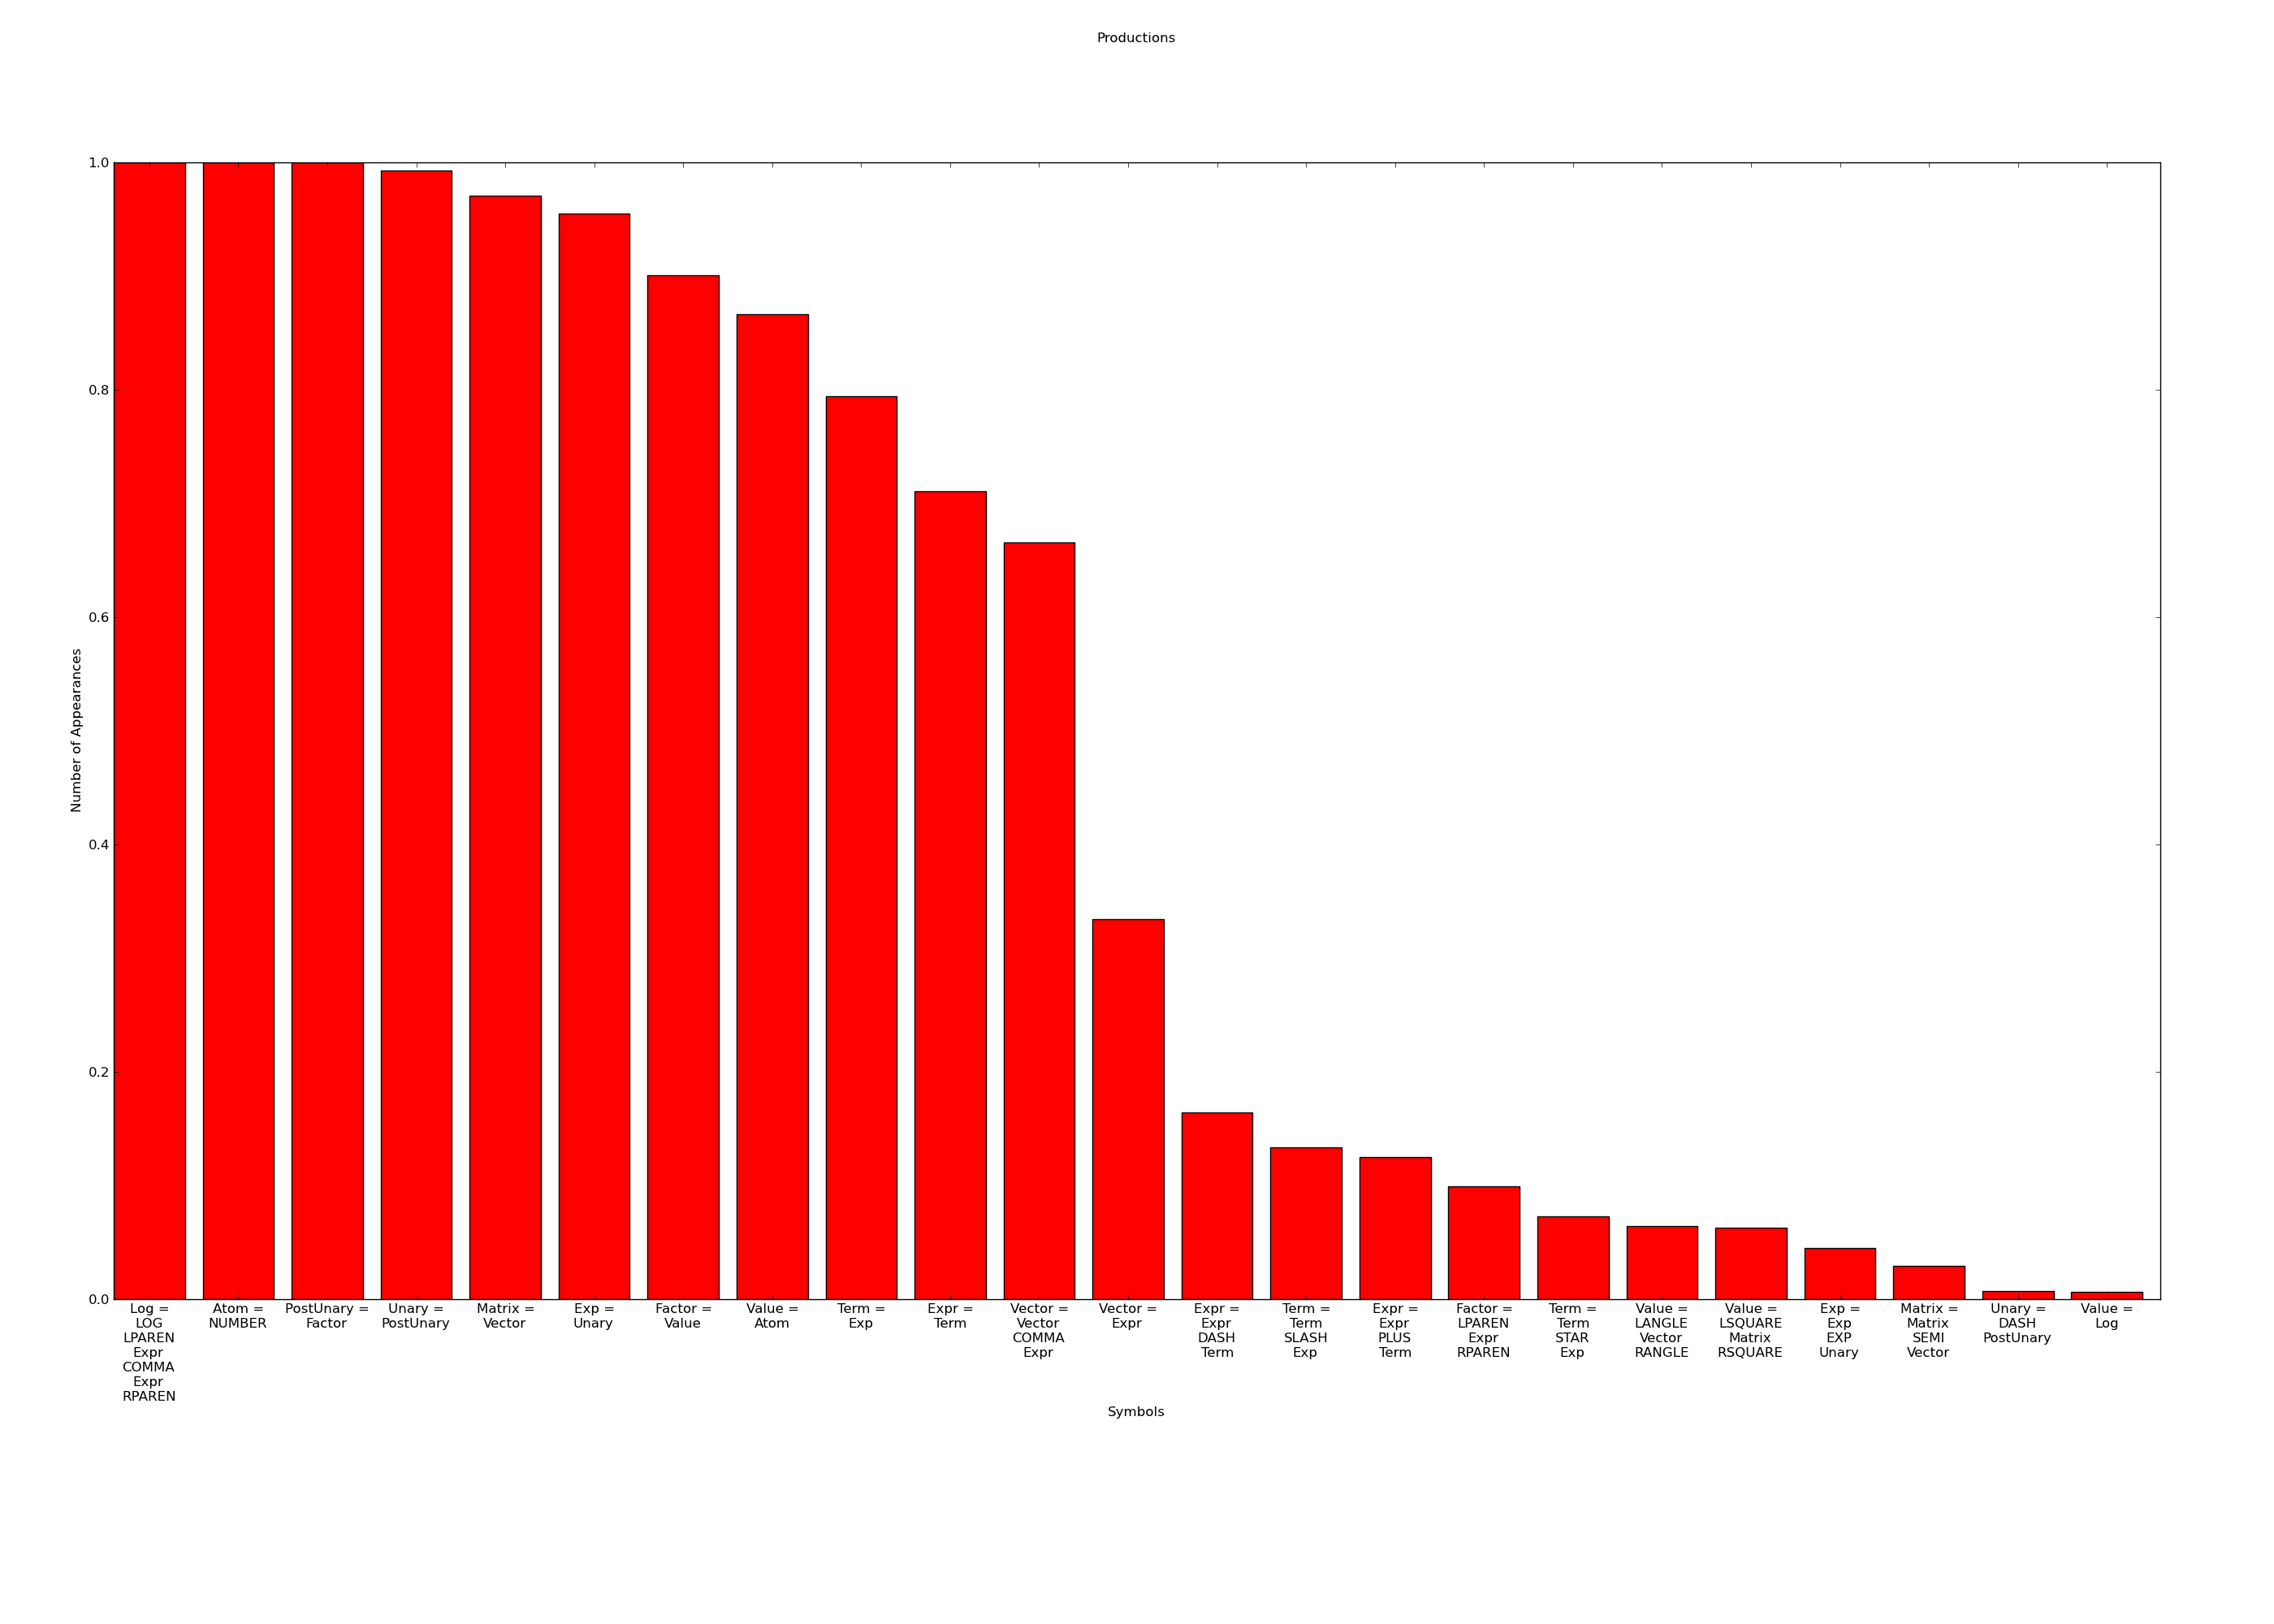
\includegraphics[scale=0.23]{figs/human/production_probability_histogram.png}
    \end{center}
        \caption{Production probability histogram when using a human corpus of
190 example inputs for a calculator program.}
    \label{times}
\end{figure*}

\begin{figure*}
    \begin{center}

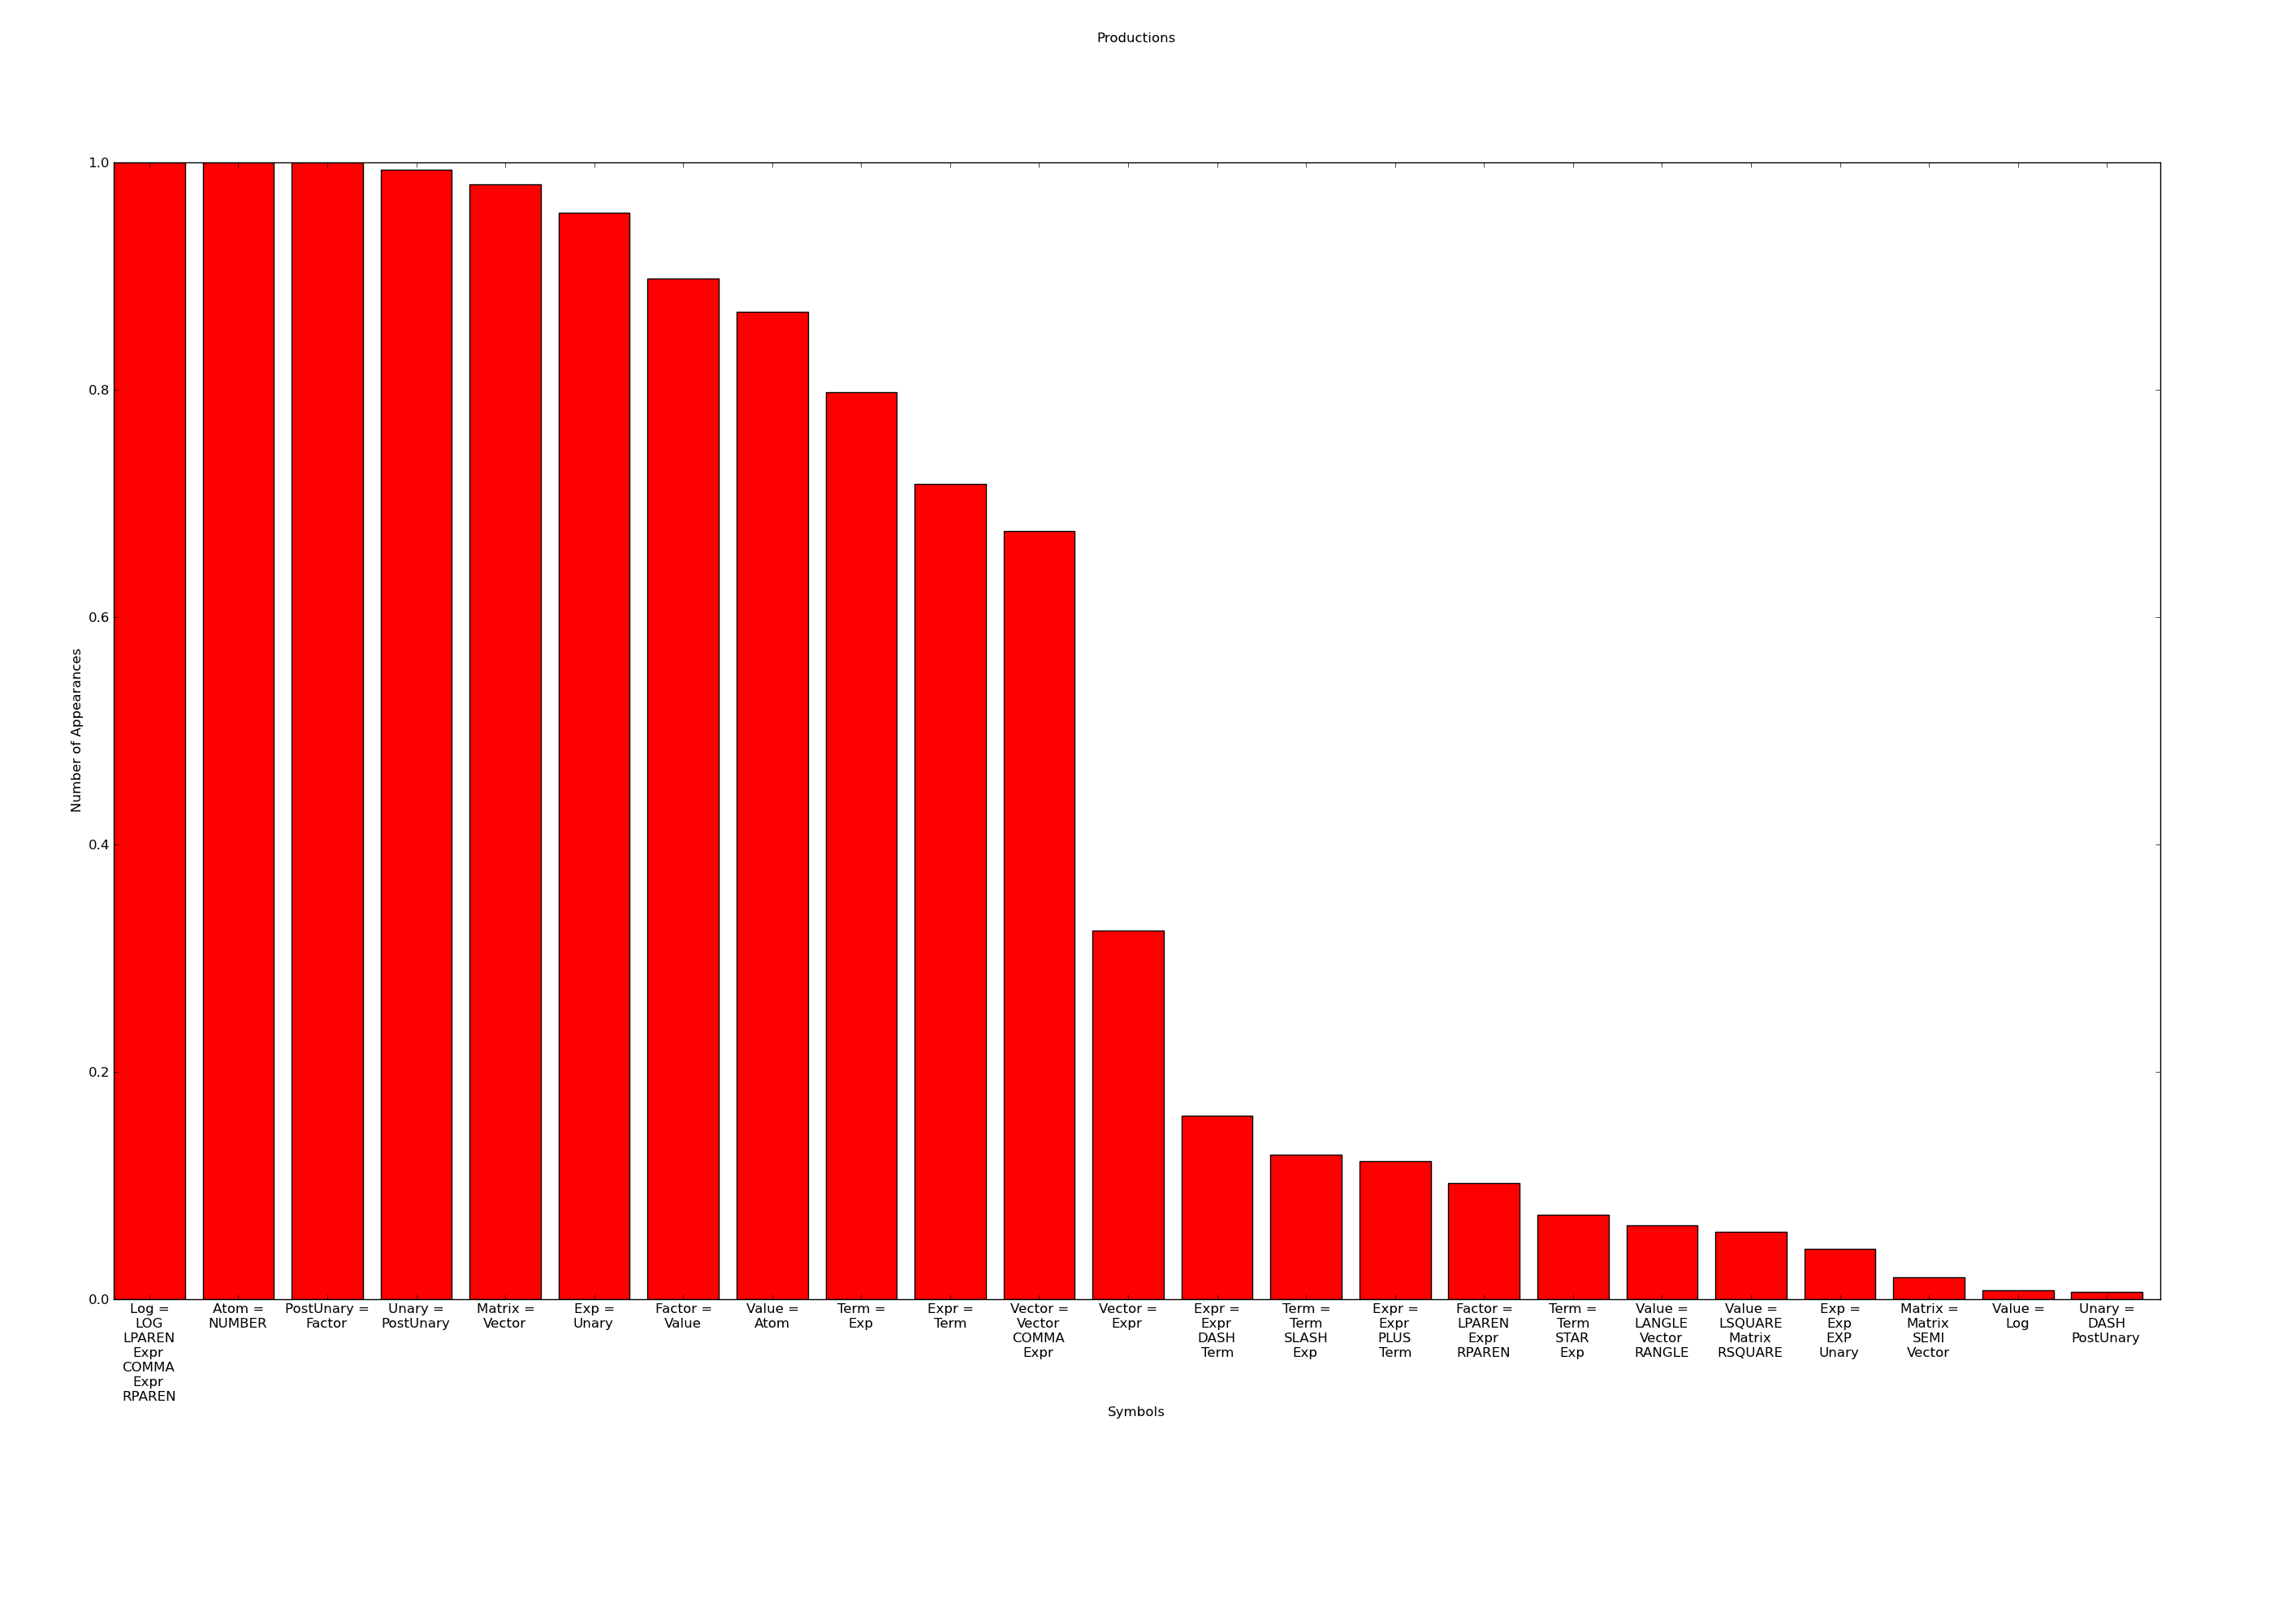
\includegraphics[scale=0.23]{figs/gen/pp/production_probability_histogram.png}
    \end{center}
        \caption{Production probability histogram when using production
probabilities
to generate an artificial corpus of 400 example inputs for a calculator
program.}
    \label{times}
\end{figure*}

\begin{figure*}
    \begin{center}

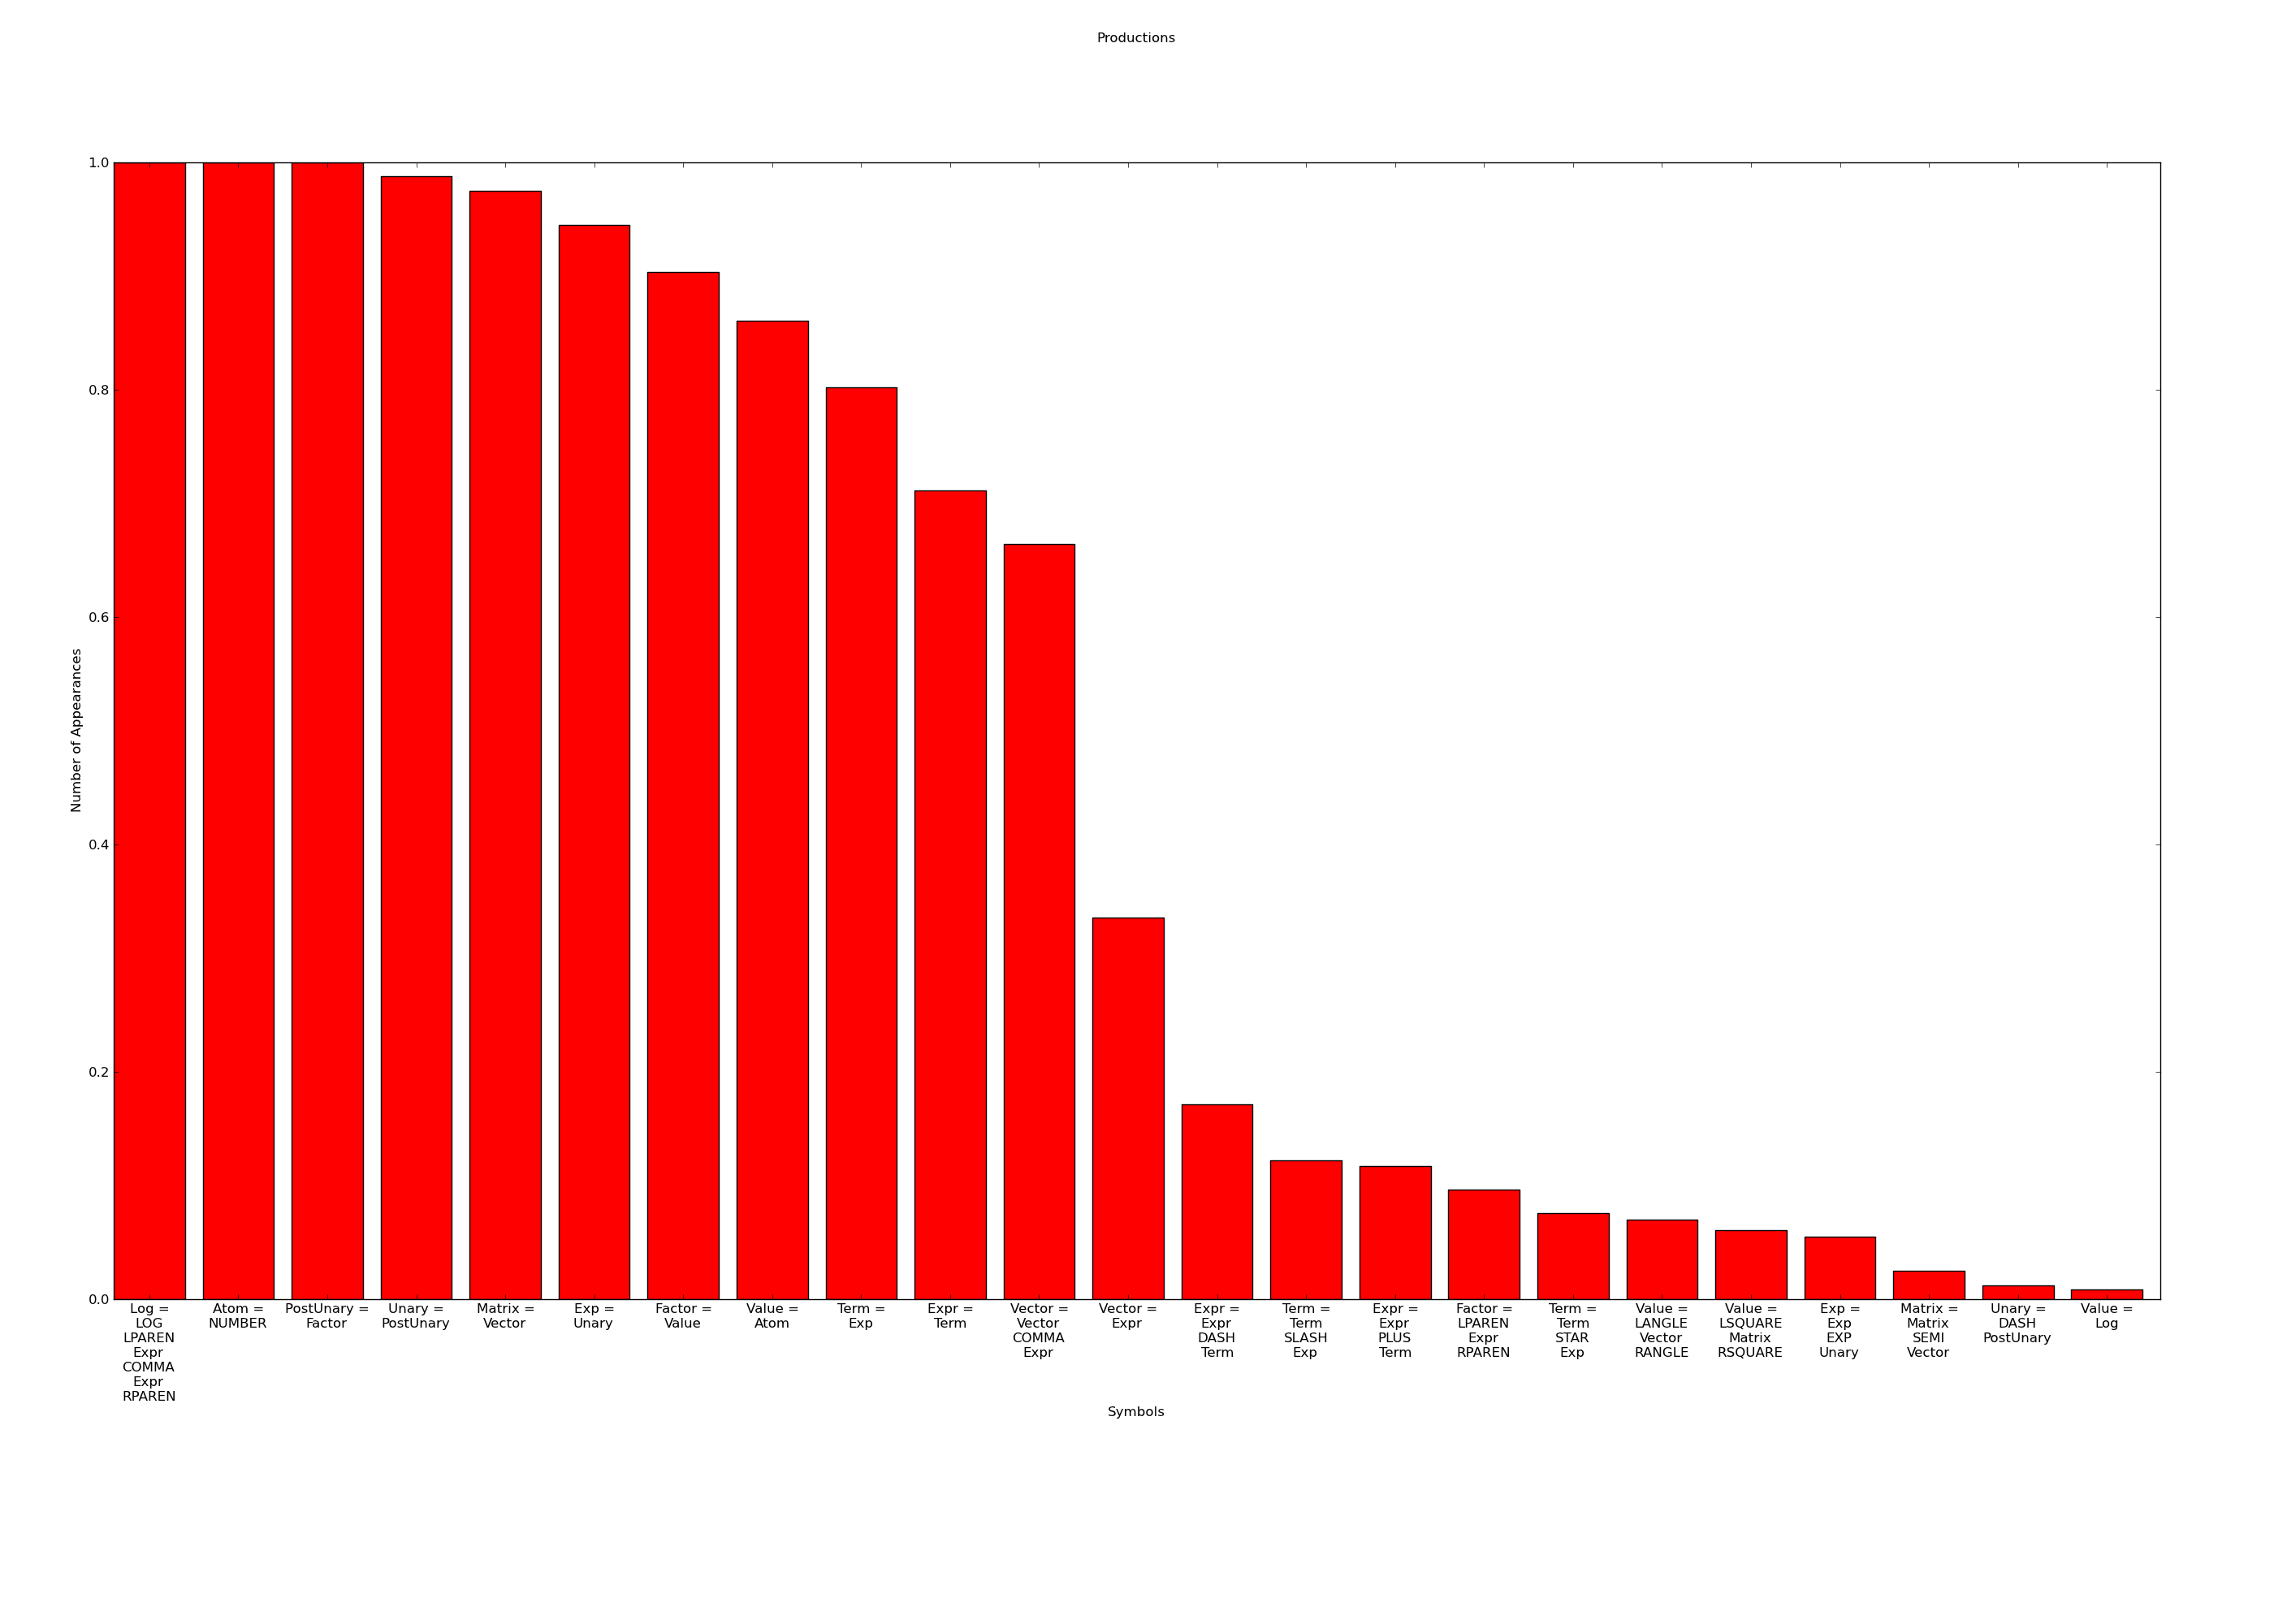
\includegraphics[scale=0.23]{figs/gen/production_probability_histogram.png}
    \end{center}
        \caption{Production probability histogram when using conditional
probabilities to generate an artificial corpus of 400 example inputs for a
calculator program.}
    \label{times}
\end{figure*}


There is no immediate difference between these three graphs. Upon closer
inspection however, differences between the example input sets are evident. Let
us examine the statistics for the $Exp => Exp:EXP:Unary$ rule from the
calculator grammar.

The human corpus produced the following 3 conditional probabilities: \\

\noindent
\begin{verbatim}
2, Exp => Exp:EXP:Unary, Expr, Term, 0.0745580322829
2, Exp => Exp:EXP:Unary, Term, Exp, 0.01398603413986
2, Exp => Exp:EXP:Unary, Term, Term, 0.00726744186047
\end{verbatim}


The artificial corpus generated using production probabilities produced the
following 13 conditional probabilities: \\

\noindent
\begin{verbatim}
2, Exp => Exp:EXP:Unary, Expr, Expr, 0.2
2, Exp => Exp:EXP:Unary, Expr, Term, 0.0460969044415
2, Exp => Exp:EXP:Unary, Exp, Term, 0.0289855072464
2, Exp => Exp:EXP:Unary, Factor, Expr, 0.037037037037
2, Exp => Exp:EXP:Unary, Factor, Term, 0.0485436893204
2, Exp => Exp:EXP:Unary, Factor, Value, 0.103448275862
2, Exp => Exp:EXP:Unary, PostUnary, Factor, 0.0581395348837
2, Exp => Exp:EXP:Unary, Term, Exp, 0.052380952381
2, Exp => Exp:EXP:Unary, Term, Term, 0.0328888888889
2, Exp => Exp:EXP:Unary, Value, Vector, 0.166666666667
2, Exp => Exp:EXP:Unary, Vector, Expr, 0.3
2, Exp => Exp:EXP:Unary, Vector, Term, 0.166666666667
2, Exp => Exp:EXP:Unary, Vector, Vector, 1.0
\end{verbatim}

The artificial corpus generated using conditional probabilities produced the
following 10 conditional probabilities: \\

\noindent
\begin{verbatim}
2, Exp => Exp:EXP:Unary, Exp, Exp, 0.0454545454545
2, Exp => Exp:EXP:Unary, Expr, Exp, 0.6
2, Exp => Exp:EXP:Unary, Expr, Term, 0.076048951049
2, Exp => Exp:EXP:Unary, Factor, Exp, 0.416666666667
2, Exp => Exp:EXP:Unary, Factor, Term, 0.384615384615
2, Exp => Exp:EXP:Unary, PostUnary, Factor, 0.458333333333
2, Exp => Exp:EXP:Unary, Term, Exp, 0.0211480362538
2, Exp => Exp:EXP:Unary, Term, Expr, 0.166666666667
2, Exp => Exp:EXP:Unary, Term, Term, 0.00593667546174
2, Exp => Exp:EXP:Unary, Vector, Expr, 0.4
\end{verbatim}

Neither of the two artificial example inputs conform closely to the
original human corpus for the $Exp => Exp:EXP:Unary$ rule. Similar results are
obtained when comparing other rules. Nevertheless, the example input generated
by using conditional probabilities is better than the one with production
probabilities as it removed 3 probabilities which should not have existed in
the first place. For example, the human corpus will only ever pick this rule if
the previous two non-terminals are $Expr, Term$ or $Term, Exp$ or $Term, Term$.
On the other hand, the corpus generated with production probabilities has a
probability for when the previous two non-terminals are $Vector, Vector$. This
probability is at least eliminated in the corpus generated with conditional
probabilities, though this corpus retains the probability for when the previous
non-terminals were $Vector, Expr$. However, it has a higher probability
than the corresponding probability in the other corpus meaning that the
conditional probabilities table removed a $Vector, Expr$ probability for some
other rule involving the $Exp$ non-terminal.

This example is particularly harsh. By examining the full tables in the
appendix, one will realize that while the artificial examples consistently
have additional probabilities than the human corpus, the difference is not
always so substantial and even better, often times conditional probabilities
will be significantly more accurate than production probabilities.

These results confirm that using conditional probabilities to generate fuzzed
output will result in more accurate test files than if one were to use
production probabilities. Nevertheless, there is clearly room for improvement:
in addition to adding different forms of statistics (see Future Work), there
are two reasons as to why the generated input includes probabilities which are
not in the human input. First, the CFGStats engine does not take semantic
constrains into account like the attribute grammar does which causes illegal
choices to be made when generating output. The human corpus consists of
semantically correct inputs. Second, the CFGStats engine does not currently
have an ``intelligent'' fall-back for when the current iteration's previous N
non-terminals do not match any provided in the table: it will pick a random
rule. The Future Work section describes better approaches to dealing with this
problem.


















\section{Using Attribute Grammars to Generate Test Cases}
\label{attrgram}

Statistically driven algorithms for context free grammars can generate examples
which mimic an input corpus from the perspective of the probability
distributions. However, even though CFG algorithms will still generate many
invalid inputs. These inputs while \textit{syntactically} correct are
\textit{semantically} incorrect. To address this issue we add semantic
constraints using attribute grammars.

\subsection{Attribute Grammars}

An attribute grammar\footnote{Sometimes these are referred to as attributed
grammars} adds context sensitive constraints onto a context free grammar.
These constraints are added by attaching to each grammar rule an option
``action'' statement and ``condition'' statement. The reader may be familiar
with attribute grammars containing only action statements (and no condition
statements) from using parser generators such as Yacc. For example the following
grammar computes the value of a simple arithmetic expression using an attributed
grammar:

\begin{verbatim}
Term -> Term PLUS Factor
        with Action {
          Term{1}.value = Term{2}.value + Factor.value
        }
      | Term DASH Factor
        with Action {
          Term{1}.value = Term{2}.value - Factor.value
        }
      | Factor
        with Action {
          Term{1}.value = Factor.value
        }
      ;
Factor -> NUMBER 
          with Action {
            Factor.value = NUMBER
          }
        ;
\end{verbatim}

\noindent
all the attributes in this example are \textit{synthesized} attributes.
Synthesized attributes are computed from the bottom up. In contrast inherited
attributes are computed from the top down.\cite{Aho2007}

\begin{figure*}
  \begin{center}
    \subfigure[CFG Parse]{
      \includegraphics[scale=0.3]{figs/ast_1.png}
      \label{ast_1}
    }
    \subfigure[Attributed CFG Parse]{
      \includegraphics[scale=0.3]{figs/ast_2.png}
      \label{ast_2}
    }
  \end{center}
  \caption{Parse trees for ``3+5''}
  \label{asts}
\end{figure*}

To understand how the grammar works an example is in order. Consider the
sentence ``3+5'' whose parse trees are given in figure \ref{asts}. The context
free parse, figure \ref{ast_1}, shows the structure of a bottom up parse of the
example. Executing the actions annotates the parse tree and produces the second
parse tree, figure \ref{ast_2}.\footnote{this is sometimes called syntax
directed translation} 

Attribute grammars of this form are often used as part of a compilation tool
chain. Indeed, they were originally designed with such a purpose in mind.
However, when conditions are added attribute grammar describe can describe
context sensitive restrictions.\cite{Slonneger1995} As an example, lets add a
constraint to our example grammar to prevent terms from holding negative values:

\begin{verbatim}
Term -> Term PLUS Factor
        with Action {
          Term{1}.value = Term{2}.value + Factor.value
        }
      | Term DASH Factor
        with Action {
          Term{1}.value = Term{2}.value - Factor.value
        }
        with Condition {
          Term{2}.value >= Factor.value
        }
      | Factor
        with Action {
          Term{1}.value = Factor.value
        }
      ;
Factor -> NUMBER 
          with Action {
            Factor.value = NUMBER
          }
        ;
\end{verbatim}

\noindent
A ``condition'' clause was added to the rule ``Term $\rightarrow$ Term DASH
Factor'' which checks to make sure the ``Term'' is always greater or equal to
the Factor. When this condition is false a parse error would occur during a
parse. For example the sentence ``5 - 10'' would no longer parse.



Example Grammar Here

Example Derivation

Generation Algorithm



\section{Mutation Fuzzing with CFG Stats and Attribute Grammars}

\subsection{Introduction}
Mutation fuzzing is a useful category of fuzzing in its ability to
generate output that is similar to existing samples. These outputs can
then be used as inputs to a program for the purpose of detecting
faults.

Mutation fuzzing is often used to generate a large set of mutants
surrounding a singular example. For practical purposes, these mutant
sets are pruned by use of various heuristics, to obtain a mutant set
which can be executed in a reasonable amount of time.

\subsection{Literature Survey}
Jia and Harman in their 2010 paper survey the general techniques used
for pruning the mutant set.\cite{Jia2010} These techniques evaluate
mutations based on what tests ``kill'' them. A test T is said to kill
a mutation M if for source S, T(S) does not give the same output as
T(M). If S and M match on T, then M is said to have ``survived''. This
evaluation method unfortunately has one serious flaw, in the form of
an undecidable problem. In some instances, mutants may be generated
that are semantically the same, but syntactically different. Due to
the undecidibility of program equivalence, it is impossible to detect
these cases. Jia recognizes this problem as being a major hindering
factor in the use of mutation fuzzing. A secondary main factor is the
need for human interaction, both as a human oracle and as a mediator
for the mutant equivalence problem.

In Jia's paper, four separate techniques for mutation set pruning are
discussed. The simplest of their surveyed techniques is to simply to
pick from the set at random. While effective at pruning, this
technique clearly lacks any ability to select the best mutants from
the set. As a step up from random selection, clustering has been
proposed as an improved pruning method. Using clustering, samples can
be selected from each cluster in order to maintain a wide range of
mutations. This clustering process is implemented by grouping
mutations that are killed by the same set of tests.
% TODO: Possibly go into Hussain's master thesis here?

The two remaining techniques attempt to use more complicated methods
to prune. The first of these, selective mutation, constrains the number
of mutations. Some mutation operations may produce excessive or
redundant mutants. By eliminating these mutations, the generated set
of mutants starts out small, largely eliminating the need for further
reductions.

The fourth and final technique discussed  by Jia and Harman is that of
Higher Order Mutation (HOM). As opposed to most mutations, which fall
into the category of First Order Mutations (FOM), HOMs are generated
by applying mutation operators multiple times.





\subsection{Results}

In Fuzzbuzz, we decided to develop mutation fuzzing as a compliment to
the CFG stat and attribute grammar methods. Usage of these three
techniques in conjunction is not a widely explored area. We predict
that these techniques will better prune the mutation space as compared
to other contemporary pruning methods.

Our work on mutation fuzzing did not extend as far as we wanted, but
it certainly set a firm foundation for future work. Support was added
to Fuzzbuzz for basic mutation based on the random selection
algorithm. Fuzzbuzz mutates nonterminals inside of the example AST in
order to produce the final result.

The current implementation is split into two easily extensible
functions. The first of these is the selection function. This function
decides what subtree of the AST should be mutated. While a simplistic
algorithm is currently employed, the system allows for the selection
function to be easily swapped out. The second important function is
the generator function. This function generates a subtree for the
given non-terminal. This part in particular is where the CFG stat and
attribute grammar implementations become very useful. While not
currently implemented as such, these two tree generation techniques
can be used for better mutation generation.



\section{Future Work}
\subsection{Attribute Grammar}
future work blah
\subsubsection{Annotating Context Free Grammars with Attributes}

Context free grammars can be annotated with synthesized attributes using a
straight forward process if the types of attributes are reasonably restricted.
For this paper we allow three types of attributes: 1) production choice, eg.
which production for the non-terminal was chosen, 2) scalar attributes, eg. the
value of a token or the name of a token, 3) set attributes, eg. collections of
scalar attributes. 

why the restrictions are reasonable 

exact bound on what can be expressed

\paragraph{Algorithm Sketch}

All possible attributes are synthesized

Conditions are proposed based, and tested against operational inputs. Only those
conditions which pass all operational inputs are kept.

Attributes un-used by final conditions are pruned.

\subsection{CFG Stats}
blargh
\subsection{Mutation Fuzzing}
The current implementation of mutation fuzzing in Fuzzbuzz is a great
foundation for future work. There is a clear path to integrating CFG
stats and attribute grammars into the generation process. By
integrating these methods, it is likely that Fuzzbuzz will be able to
prune the mutation space to sufficient level to generate mutations
that are effective at fault discovery.

\section{Conclusion}
Hello, this project is good.

This project is a work in progress

We have discovered that this solution is good from a blackbox
perspective.


%-----------------------------------

Fuzzbuzz explores a wide range of fuzzing techniques. However, it is
still very much a work in progres. While it is not yet a
fully featured fuzzing framework, it still provides a valuable toolset
for anyone interested in fuzz testing.

Tim will now talk about blackbox stuff.




\bibliographystyle{acm}
\bibliography{bibliography}

\appendix

\section{This is a Hard Problem}
\label{hard}

Generating strings from an attribute grammar is NP-Complete.

\subparagraph{Outline}

\begin{enumerate}[1.]
\item
  Reduction 3SAT -\textgreater{} AGSG {[}Shows AGSG at least NP-Hard{]}
\item
  Proof of Poly-Time Verifiable Certificate {[}AGSG in NP{]}
\end{enumerate}
Since AGSG is NP-Hard and it is in NP it is NP-Complete.

\subsubsection{Decision Problem}

Is the language generated by this grammar the empty language?

\subsection{Reduction, 3SAT -\textgreater{} AGSG {[}Attribute Grammar
String Generation{]}}

\subsubsection{Construct a grammar for the 3SAT instance}

eg.

\begin{verbatim}
(x1 || x2 || x3) && (x2 || ~x3 || x4) ... (x2 || x3 || x4)
\end{verbatim}
becomes

\begin{verbatim}
SAT -> AndsM ;

AndM -> AndsM-1 AND ClauseM ;
...
And2 -> Ands1 AND Clause2 ;
And1 -> Clause1 ;

Clause1 -> '(' x1 OR x2 OR x3 ')' ;
Clause2 -> '(' x2 OR NOT x3 OR x4 ')' ;
...
ClauseM -> '(' x2 OR x3 OR x4 ')' ;

x1 -> TRUE
    | FALSE
    ;
x2 -> TRUE
    g| FALSE
    ;
...
xN -> TRUE
    | FALSE
    ;
\engd{verbatim}
With attributes which synthesize the values for each clause and with a
condition which asserts that the whole expression is true.

\begin{verbatim}
SAT -> AndsM
       with Condition {
         AndsM.value == True
       }
       ;

AndM -> AndsM-1 AND ClauseM
         with Action {
            AndsM.value = AndM-1.value && ClauseM.value
            AndsM.names = {
              ClauseM.a.name:ClauseM.a.value,
              ClauseM.b.name:ClauseM.b.value,
              ClauseM.c.name:ClauseM.c.value
            }
            AndsM.names = AndsM.names | AndsM-1.names
         }
         with Condition {
           (ClauseM.a.name != ClauseM.b.name ||
             ClauseM.a.value == ClauseM.b.value) &&
           (ClauseM.c.name != ClauseM.b.name ||
             ClauseM.c.value == ClauseM.b.value) &&
           (ClauseM.a.name != ClauseM.c.name ||
             ClauseM.a.value == ClauseM.c.value) &&
           (ClauseM.a.name not in AndsM-1.names ||
             ClauseM.a.value == AndsM-1.names[ClauseM.a.name]) &&
           (ClauseM.b.name not in AndsM-1.names ||
             ClauseM.b.value == AndsM-1.names[ClauseM.b.name]) &&
           (ClauseM.c.name not in AndsM-1.names ||
             ClauseM.c.value == AndsM-1.names[ClauseM.c.name])
         }
         ;
...
And2 -> Ands1 AND Clause2
         with Action {
            Ands2.value = Ands1.value && Clause2.value
            Ands2.names = {
              Clause2.a.name:Clause2.a.value,
              Clause2.b.name:Clause2.b.value,
              Clause2.c.name:Clause2.c.value
            }
            Ands2.names = Ands2.names | Ands1.names
         }
         with Condition {
           (Clause2.a.name != Clause2.b.name ||
             Clause2.a.value == Clause2.b.value) &&
           (Clause2.c.name != Clause2.b.name ||
             Clause2.c.value == Clause2.b.value) &&
           (Clause2.a.name != Clause2.c.name ||
             Clause2.a.value == Clause2.c.value) &&
           (Clause2.a.name not in Ands1.names ||
             Clause2.a.value == Ands1.names[Clause2.a.name]) &&
           (Clause2.b.name not in Ands1.names ||
             Clause2.b.value == Ands1.names[Clause2.b.name]) &&
           (Clause2.c.name not in Ands1.names ||
             Clause2.c.value == Ands1.names[Clause2.c.name])
         }
         ;
And1 -> Clause1
         with Action {
            Ands1.value = Clause1.value
            Ands1.names = {
              Clause1.a.name:Clause1.a.value,
              Clause1.b.name:Clause1.b.value,
              Clause1.c.name:Clause1.c.value
            }
         }
         with Condition {
           (Clause1.a.name != Clause1.b.name ||
             Clause1.a.value == Clause1.b.value) &&
           (Clause1.c.name != Clause1.b.name ||
             Clause1.c.value == Clause1.b.value) &&
           (Clause1.a.name != Clause1.c.name ||
             Clause1.a.value == Clause1.c.value)
         }
         ;

Clause1 -> '(' x1 OR x2 OR x3 ')'
           with Action {
             Clause1.value = x1.value || x2.value || x3.value
             Clause1.a.name = 'x1'
             Clause1.a.value = x1.value
             Clause1.b.name = 'x2'
             Clause1.b.value = x2.value
             Clause1.c.name = 'x3'
             Clause1.c.value = x3.value
           }
           ;
Clause2 -> '(' x2 OR NOT x3 OR x4 ')'
           with Action {
             Clause2.value = x2.value || !x3.value || x4.value
             Clause2.a.name = 'x2'
             Clause2.a.value = x2.value
             Clause2.b.name = 'x3'
             Clause2.b.value = x3.value
             Clause2.c.name = 'x4'
             Clause2.c.value = x4.value
           }
           ;
...
ClauseM -> '(' x2 OR x3 OR x4 ')'
           with Action {
             ClauseM.value = x2.value || x3.value || x4.value
             ClauseM.a.name = 'x2'
             ClauseM.a.value = x2.value
             ClauseM.b.name = 'x3'
             ClauseM.b.value = x3.value
             ClauseM.c.name = 'x4'
             ClauseM.c.value = x4.value
           }
           ;

x1 -> TRUE
      with Action {
        x1.value = True
      }
    | FALSE
      with Action {
        x1.value = False
      }
    ;
x2 -> TRUE
      with Action {
        x1.value = True
      }
    | False
      with Action {
        x1.value = False
      }
    ;
...
xN -> TRUE
      with Action {
        x1.value = True
      }
    | FALSE
      with Action {
        x1.value = False
      }
    ;
\end{verbatim}
This translation from 3SAT to AGSG is clearly poly time.
O(\textbar{}C\textbar{} + \textbar{}V\textbar{}) where C = the clauses
in 3SAT and V = the variables.

\subsubsection{Show a solution for 3SAT ---\textgreater{} creates a
parsable string for AGSG}

In a solution for 3SAT all names (x1, x2, \ldots{} xN) always have
exactly one value (True or False) assigned to them. The condition on
each ``AndX'' production {[}And1, And2 \ldots{}{]} states that each name
always has the same value. That is once xN has recieved a value (True or
False) all other instances of xN must have the same value. Therefore,
all conditions are the AndX clauses are satisfied by any solution to
3SAT by the definition of a 3SAT solution.

The actions on each variable production (x1, x2, \ldots{} xN) produce a
value, eg. \verb!x1.value!, either equal to True or False. The actions
on each clause production (Clause1, Clause2, \ldots{} ClauseN) combine
the values of the variables in that clause together. They combine them
in the same way they are combined in the equivalent clause in 3SAT by
construction.

Finally the chain of And productions (And1, And2, \ldots{} AndN) combine
the values synthesized by the clauses (\verb!Clause1.value!,
\verb!Clause2.value!, \ldots{} \verb!ClauseN.value!). Into a final value
\verb!AndN.value! via:

\begin{verbatim}
And1.value = Clause1.value
And2.value = And1.value && Clause2.value
And3.value = And2.value && Clause3.value
...
AndN.value = AndN-1.value && ClauseN.value
\end{verbatim}
which can be reduced to 1 expression with algebraic substitution as:

\begin{verbatim}
AndN.value = Clause1.value && Clause2.value && ... && ClauseN.value
\end{verbatim}
Which synthesizes the same value which the 3SAT problem specifies. Once
again by construction.

Therefore, if a variable assignment satisfies 3SAT then it must also
synthesize a value of \verb!True! on \verb!AndN.value! resulting in a
parsable expression.

\subsubsection{Show a string generated by the grammar ---\textgreater{}
is a solution for 3SAT}

In the above proof, we showed that the attributes on the grammar compute
the same answer as algebraically evaulating the 3SAT expression. Since
(once again by the above proof) there is a unique variable assignment in
the generated string this string must evaluate to True. If it didn't it
could not have been generated by the grammar. Therefore, the string
generated corresponds to a unique variable assignment in 3SAT which
causes the expression to evaluate to True.

\subsection{AGSG is in NP}

\paragraph{Certificate}

A string of terminal symbols.

\subsection{Show the Certificate can be Verified in Poly-Time}

\subsubsection{The Algorithm for Verification}

\begin{itemize}
\item
  Transform the Context-Free grammar into Chomsky Normal Form. This
  ensures a polynomial tree height with each Non-Terminal symbol having
  at most 2 children.
\item
  Using the Chomsky Normal Form Context-Free version of the grammar
  parse the string and transform it into a parse tree.
\item
  Using a Post-Order tree traversal to apply the actions and check the
  conditions of each grammar rule
\end{itemize}
\subsubsection{Proof Alg. in Poly-Time}

Since the parse tree has a polynomial number of nodes there are only a
polynomial number of steps. However, how bad can 1 of those steps be in
the worst case? That is, how much time can it take to check a condition?
Is it linear with respect to the input (which includes: the attribute
grammar, and the certificate)?

To examine this we will start with the leaves of the parse tree. Each
leaf is a Terminal Symbol. A constant number of attributes can be
produced by a single terminal symbol. We denote this number as $C$.
Therefore, there can be at most $C$ actions and $C^2 D$ terms in the
condition --- where $D$ is the number of binary comparison operators in
the language.

Most importantly, if the condition actually has $C^2 D$ terms every term
has to be written down. So checking the truth value of the condition is
linear with respect to the size of the attribute grammar. If loops or
quantifiers such as $\exists$ and $\forall$ are allowed this no longer
holds. However, since we do not allow quantification in the conditions
checking a leaf condition (and indeed any condition) must be linear with
respect to the size of the input.

At internal nodes the number of terms in a condition could be as high as
$(2^{h-2}C)^2 D$ where $h$ is the height of the subtree rooted at the
current node. Once again, while this is clearly an exponential number,
it is not exponential with respect to the input as each term is part of
the input.

\subparagraph{Therefore,}

checking all conditions are satisfied is polynomial time as long as
quantifiers are disallowed from conditions.



